\clearpage
\section{Theory}\label{sec:Theory}
The Lattice Boltzmann Equation makes use of the populations indicated by the vector $\bm{f}$. For two-dimensional simulations, we choose to have nine velocity directions, indicated by D2Q9. This means that the populations $\bm{f}$ have nine elements. The nine discrete velocity components and their respective weights are given by:

\begin{equation}\label{eq:Discrete velocity components and weights}
\begin{split}
    \left\{\bm{c}_i\right\} &= \left\{(0,0),\, (\pm 1, 0),\, (0, \pm 1),\, (\pm 1, \pm 1)\right\}\\
    \left\{w_i\right\} &= \left\{4/9,\, 1/9,\, 1/9,\, 1/9,\, 1/9,\, 1/36,\, 1/36,\, 1/36,\, 1/36\right\}
\end{split}
\end{equation}

For a single fluid component in the absence of forces, the macroscopic quanties can be computed from the populations:

\begin{equation}\label{eq:Macroscopic quantities}
\begin{split}
    \rho &= \sum_{i} f_i\\
    \bm{u} &= \frac{1}{\rho} \sum_i f_i \bm{c}_i\\
    p &= c_s^2 \rho
\end{split}
\end{equation}

Where $c_s$ is the speed of sound, with $c_s^2 = 1/3$ for the D2Q9 velocity set. 

\subsection{Lattice Boltzmann Equation}\label{subsec:Lattice Boltzmann Equation}
We can now introduce the Lattice Boltzmann Equation for a single fluid component in the absence of any sources:

\begin{equation}\label{eq:Lattice boltzmann equation}
    f_i(\bm{x} + \bm{c}_i, t+1) = f_i(\bm{x}, t) + \Omega_{i j} \Bigl(f_j(\bm{x}, t) - f_j^{\text{eq}}(\bm{x}, t)\Bigr)
\end{equation}

Where a sum over the index $j$ is implied. We already choose the timestep and the gridspacing as $\Delta t = \Delta x = 1$ as is often done. If the populations will not change anymore under collisions, they will equation the equilibrium populations given by $\bm{f}^{\text{eq}}$. This can be computed as:

\begin{equation}\label{eq:Equilibrium populations}
    f^{\text{eq}}_i = w_i \rho \left(1 + \frac{\bm{u} \cdot \bm{c}_i}{c_s^2} + \frac{{\left(\bm{u} \cdot \bm{c}_i\right)}^2}{2c_s^4} - \frac{|\bm{u}|^2}{2c_s^2}\right)
\end{equation}

Furthermore, the collision operator is given by the matrix $\bm{\Omega}$. We choose the simple BGK operator:

\begin{equation}\label{eq:Collision operator BGK}
    \bm{\Omega}_{\text{BGK}} = -\frac{1}{\tau}\bm{I}
\end{equation}

Where $\bm{I}$ is the identity matrix and $\tau$ is the relaxation time, which is related to the kinematic viscosity of the fluid as:

\begin{equation}\label{eq:Kinetmatic viscosity}
    \nu = c_s^2 \left(\tau - \frac{1}{2}\right)
\end{equation}

\subsection{Collision and streaming}\label{eq:Collision and streaming}
The Lattice Boltzmann equation~\ref{eq:Lattice boltzmann equation} can be split up in a collision step and a streaming step. The collision step is given by:

\begin{equation}\label{eq:Collision step}
    \bm{f}^*(\bm{x}, t) = \bm{f}(\bm{x}, t) - \frac{1}{\tau}\Bigl( \bm{f}(\bm{x}, t) - \bm{f}^{\text{eq}}(\bm{x}, t) \Bigr)
\end{equation}

And the streaming step is given by:

\begin{equation}\label{eq:Streaming step}
    f_i(\bm{x}, t+1) = f_i^*(\bm{x} - \bm{c}_i, t)
\end{equation}

Which together are equivalent to equation~\ref{eq:Lattice boltzmann equation}.

\subsection{Boundary conditions}\label{subsec:Boundary conditions}
During the streaming step in equation~\ref{eq:Streaming step}, it is possible that the vector $\bm{x} - \bm{c}_i$ will be outside of the domain. When this happens, we will apply the suitable boundary conditions. When the crossed boundary is periodic, the streaming step can be written as:

\begin{equation}\label{eq:Periodic streaming step}
    f_i(\bm{x}, t+1) = f_i^*(\bm{x} - \bm{c}_i \mod \bm{L} , t)
\end{equation}

Where $\bm{L}$ is a vector containing the sidelengths of the domain. When the crossed boundary is a no-slip boundary, we will make use of the half-way bounce-back scheme. We assume that the wall is half a gridpoint removed from the outermost gridpoints. During the streaming step, the populations will hit the wall at $t + 1/2$ and return to the original gridpoint at $t + 1$, with inverse velocity:

\begin{equation}\label{eq:No-slip streaming step}
    f_i(\bm{x}, t+1) = f_q^*(\bm{x}, t)
\end{equation}

Where the index $q$ is given by:

\begin{equation}\label{eq:Bounce-back velocity component}
    \bm{c}_q = -\bm{c}_i
\end{equation}

We can also have open boundaries. We can impose 

\subsection{Basic algorithm}\label{subsec:Basic algorithm}
The basic algorithm for a single component without any sources, given by the Lattice Boltzmann equation~\ref{eq:Lattice boltzmann equation}, can be desribed as follows:

\begin{itemize}\label{it:Basic algorithm}
    \item[(i)] Choose $\rho(t=0)$ and $\bm{u}(t=0)$.
    \item[(ii)] Initialize the populations as $\bm{f}(t=0) = \bm{f}^{\text{eq}}(\rho, \bm{u})$. 
    \item[1] Calculate $\bm{f}^{\text{eq}}(\rho, \bm{u})$.
    \item[2] Collide the populations $\rightarrow$ $\bm{f}^*$.
    \item[3] Stream the populations $\rightarrow$ $\bm{f}(t + 1)$.
    \item[4] Calculate macroscopic quantities $\rho(t + 1)$ and $\bm{u}(t + 1)$.
    \item[5] $t = t + 1$ and return to step 1 while $t < t_{\text{final}}$.
\end{itemize}

\subsection{Sources}
When forces are applied on the fluid, the right hand side of the Lattice Boltzmann Equation in equation~\ref{eq:Lattice boltzmann equation} contains a source term $S_i$. We compute this source term from the applied force field $\bm{F}(\bm{x}, t)$ as:

\begin{equation}\label{eq:Source term}
    S_i(\bm{x}, t) = \left(1 - \frac{1}{2\tau}\right) w_i \left(\frac{\bm{c}_i - \bm{u}(\bm{x}, t)}{c_s^2} + \frac{\bm{c}_i \cdot \bm{u}(\bm{x}, t)}{c_s^4}\bm{c}_i\right) \cdot \bm{F}(\bm{x}, t)
\end{equation}

Note that a correction is added for the computation of the velocity field:

\begin{equation}\label{eq:Velocity with correction}
    \bm{u} = \frac{1}{\rho} \left(\sum_i f_i \bm{c}_i + \frac{1}{2}\bm{F}\right)
\end{equation}

Finally, we choose an initial density and velocity field at the start of the equation, as shown in the basic algorithm~\ref{subsec:Basic algorithm}. However, the computation of $\bm{u}$ requires the force $\bm{F}$ to be incorporated. The velocity field that will be used during the first step is given by:

\begin{equation}
    \bm{u} = \bm{u}_0 - \frac{\bm{F}}{2\rho}
\end{equation}

\subsection{Algorithm with sources}
The algorithm for a single component with a sources, given by the Lattice Boltzmann Equation~\ref{eq:Lattice boltzmann equation} with a source $S_i$, can be described as follows:

\begin{itemize}\label{it:Algorithm with sources}
    \item[(i)] Determine $\bm{F}(t=0)$.
    \item[(ii)] Choose $\rho(t=0)$ and $\bm{u}_0$ and compute $\bm{u}$.
    \item[(iii)] Initialize the populations as $\bm{f}(t=0) = \bm{f}^{\text{eq}}(\rho, \bm{u})$. 
    \item[1] Calculate $\bm{f}^{\text{eq}}(\rho, \bm{u})$.
    \item[2] Calculate source $S_i$.
    \item[3] Collide the populations $\rightarrow$ $\bm{f}^*$.
    \item[4] Stream the populations $\rightarrow$ $\bm{f}(t + 1)$.
    \item[5] Determine $\bm{F}(t + 1)$.
    \item[6] Calculate macroscopic quantities $\rho(t + 1)$ and $\bm{u}(t + 1)$.
    \item[7] $t = t + 1$ and return to step 1 while $t < t_{\text{final}}$.
\end{itemize}

\subsection{Poiseuille flow}
We can test the algorithm given in~\ref{it:Algorithm with sources} by making use of a two-dimensional Poiseuille flow. We use periodic boundary conditions given in equation~\ref{eq:Periodic streaming step} in the x-direction and no-slip boundary conditions given in equation~\ref{eq:No-slip streaming step} in the y-direction. The pressure gradient applied on the fluid is simulated as a body force, such that $\bm{F}(\bm{x}, t) = F_p \hat{\bm{x}}$. The initial density and velocity field are set to unity and zero, respectively. The analytical solution for this Poiseuille flow at asymptotic time is given by:

\begin{equation}
    u(y) = \frac{F_p}{2 \nu} \left( d^2 - y^2 \right)
\end{equation}

Where we defined the radius of the pipe as $d = N_y/2$ using the number of cells $N_y$ in the y-direction. Furthermore, $y_j = -d + 0.5 + j$. Using $N_x = 32$, $N_y = 128$ and $\tau = 1$, we get the result given in figure~\ref{fig:poiseuille}.

\begin{figure}[htp]
    \centering
    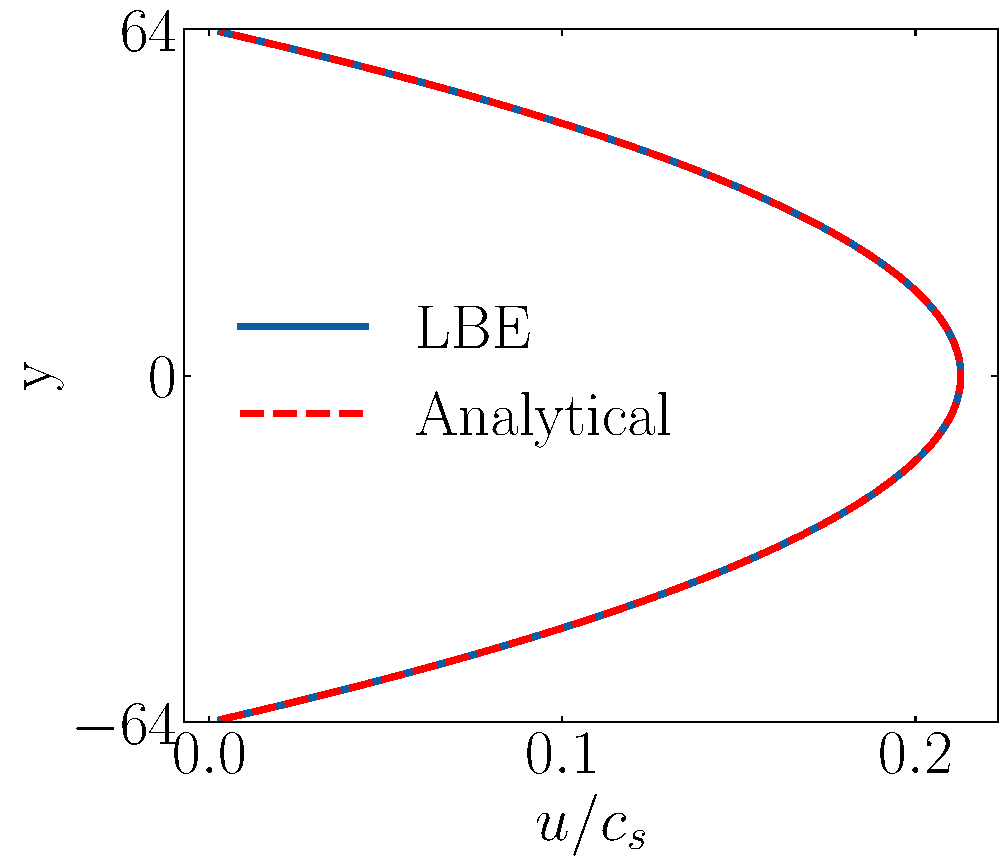
\includegraphics[width=0.5\textwidth]{figures/poiseuille.pdf}
    \caption{Flow profile of simulated Poiseuille flow at $t=10^5$ compared to the analytical solution.}\label{fig:poiseuille}
\end{figure}

\subsection{Multicomponent Shan-Chen method}
To simulate a multicomponent fluid, we extend the Lattice Boltzmann Equation as follows:

\begin{equation}\label{eq:Lattice Boltzmann Equation multicomponent}
    f_i^{\sigma}(\bm{x} + \bm{c}_i, t + 1) = f_i^{\sigma}(\bm{x}, t) - \frac{1}{\tau^{\sigma}}\Bigl(f_i^{\sigma}(\bm{x}, t) - f_i^{\text{eq}, \sigma}(\bm{x}, t)\Bigr) + S_i^{\sigma} 
\end{equation}

The fluids will exert a repelling force on each other, given by the Shan-Chen force:

\begin{equation}\label{eq:Shan-Chen force}
    \bm{F}^{\sigma}_{\text{SC}}(\bm{x}) = -G \psi^{\sigma}(\bm{x}) \sum_i \left(w_i \psi^{\sigma^\ast}(\bm{x} + \bm{c}_i) \bm{c}_i \right) 
\end{equation}

Where we assume that the individual fluids are ideal, so the fluids don't exert forces on themselves. The interaction strength is given by $G$, which should be positive for the fluids to repel each other, making them partially immiscible. Note that $\sigma^\ast$ indicates the other fluid component. The pseudopotential is given by $\psi$, which is most often given by:

\begin{equation}\label{eq:Pseudopotential}
    \psi(\rho) = \rho_0 \left(1 - e^{-\rho/\rho_0}\right) \approx \rho
\end{equation}

Where $\rho_0$ is the reference density, chosen by us to be unity in all simulations. The approximation is a first order Taylor expansion often used for the pseudopotential. The boundary conditions for the pressure in equation~\ref{eq:Shan-Chen force} are given by:

\begin{equation}
\begin{cases}
    \rho(\bm{x} + \bm{c}_i \mod\bm{L}), & \text{if periodic.}\\
    \rho(\bm{x}), & \text{if no-slip.}
\end{cases}
\end{equation}

After computing the Shan-Chen force in equation~\ref{eq:Shan-Chen force}, we can add this to the body force that we applied to find the total force on the individual fluid components. We need the individual densities and the total density to find the total force on the fluid components:

\begin{equation}\label{eq:Multicomponent densities}
\begin{split}
    \rho^\sigma &= \sum_i f_i^\sigma\\
    \rho &= \sum_\sigma \rho^\sigma
\end{split}
\end{equation}

The total force is computed as:

\begin{equation}\label{eq:Total force Shan-Chen}
    \bm{F}^\sigma = \bm{F}^\sigma_{\text{SC}} + \frac{\rho^\sigma}{\rho}\bm{F}_p
\end{equation}

The source term $S_i^\sigma$ is calculated as:

\begin{equation}\label{eq:Source term multicomponent}
    S_i^\sigma(\bm{x}, t) = \left(1 - \frac{1}{2\tau^\sigma}\right) w_i \left(\frac{\bm{c}_i - \bm{u}(\bm{x}, t)}{c_s^2} + \frac{\bm{c}_i \cdot \bm{u}(\bm{x}, t)}{c_s^4}\bm{c}_i\right) \cdot \bm{F}^\sigma(\bm{x}, t)
\end{equation}

The velocity of the total fluid is now computed as:

\begin{equation}\label{eq:Shan-Chen velocity}
    \bm{u} = \frac{1}{\rho} \sum_\sigma \left(\sum_i \left(f_i^\sigma \bm{c}_i\right) + \frac{\bm{F}^\sigma}{2}\right)
\end{equation}

Where we use the same velocity for both fluid components. For the initial condition, we again choose an initial velocity field and take into account the forcing needed for the equilibrium distributions:

\begin{equation}
    \bm{u} = \bm{u}_0 - \frac{1}{2\rho}\sum_\sigma \bm{F}^\sigma
\end{equation}

\subsection{Algorithm multicomponent Shan-Chen}
The algorithm for a multicomponent fluid with a sources, given by the Lattice Boltzmann Equation~\ref{eq:Lattice Boltzmann Equation multicomponent}

\begin{itemize}\label{it:Algorithm multicomponent Shan-Chen}
    \item[(i)] Choose $\rho(t=0)$ and $\bm{u}_0$.
    \item[(ii)] Determine $\bm{F}_{\text{SC}}^\sigma(t=0)$ and $\bm{F}^\sigma(t=0)$.
    \item[(iii)] Compute $\bm{u}$. 
    \item[(iv)] Initialize the populations as $\bm{f}^\sigma(t=0) = \bm{f}^{\text{eq}, \sigma}(\rho^\sigma, \bm{u})$. 
    \item[1] Calculate $\bm{f}^{\text{eq}, \sigma}(\rho^\sigma, \bm{u})$.
    \item[2] Calculate source $S_i^\sigma$.
    \item[3] Collide the populations $\rightarrow$ $\bm{f}^{\ast, \sigma}$.
    \item[4] Stream the populations $\rightarrow$ $\bm{f}^\sigma(t + 1)$.
    \item[5] Calculate $\rho(t + 1)$.  
    \item[6] Determine $\bm{F}_{\text{SC}}^\sigma(t+1)$ and $\bm{F}^\sigma(t+1)$.
    \item[7] Calculate $\bm{u}(t + 1)$.
    \item[8] $t = t + 1$ and return to step 1 while $t < t_{\text{final}}$.
\end{itemize}

\subsection{Multicomponent Poiseuille flow}
We can test the algorithm given in~\ref{it:Algorithm multicomponent Shan-Chen} by making use of a two-dimensional Multicomponent Poiseuille flow, where we have a high viscosity fluid at $|y| > a$ and a low viscosity fluid at $|y| < a$. The analytical solution is given by:

\begin{equation}
\begin{cases}
    u(y) = \frac{F_p}{2 \nu_{\text{high}}}\left(L_y^2 - y^2\right), & \text{for } |y| > a\\
    u(y) = \frac{F_p}{2 \nu_{\text{high}}}\left(L_y^2 - a^2\right) + \frac{F_p}{2 \nu_{\text{low}}}\left(a^2 - y^2\right), & \text{for } |y| < a
\end{cases}
\end{equation}

We now choose $a = N_y / 4$, $\nu_{\text{high}} = 1/6$, $\nu_{\text{high}} = 1/24$ and $G = 4$. This gives the result given in figure~\ref{fig:poiseuille_mc}. The velocity field is underpredicted with respect to the analyitical solution. This can be explained by the fact that the density outside of the interaction zones of the two fluids is larger than unity, to compensate the reduced mass in the interaction zones. The actual solution for the two-component Poiseuille flow contains the dynamic viscosity $\mu = \rho \nu$, which is not equal to the kinematic viscosity $\nu$ if the density is not unity. 

\begin{figure}[htp]
    \centering
    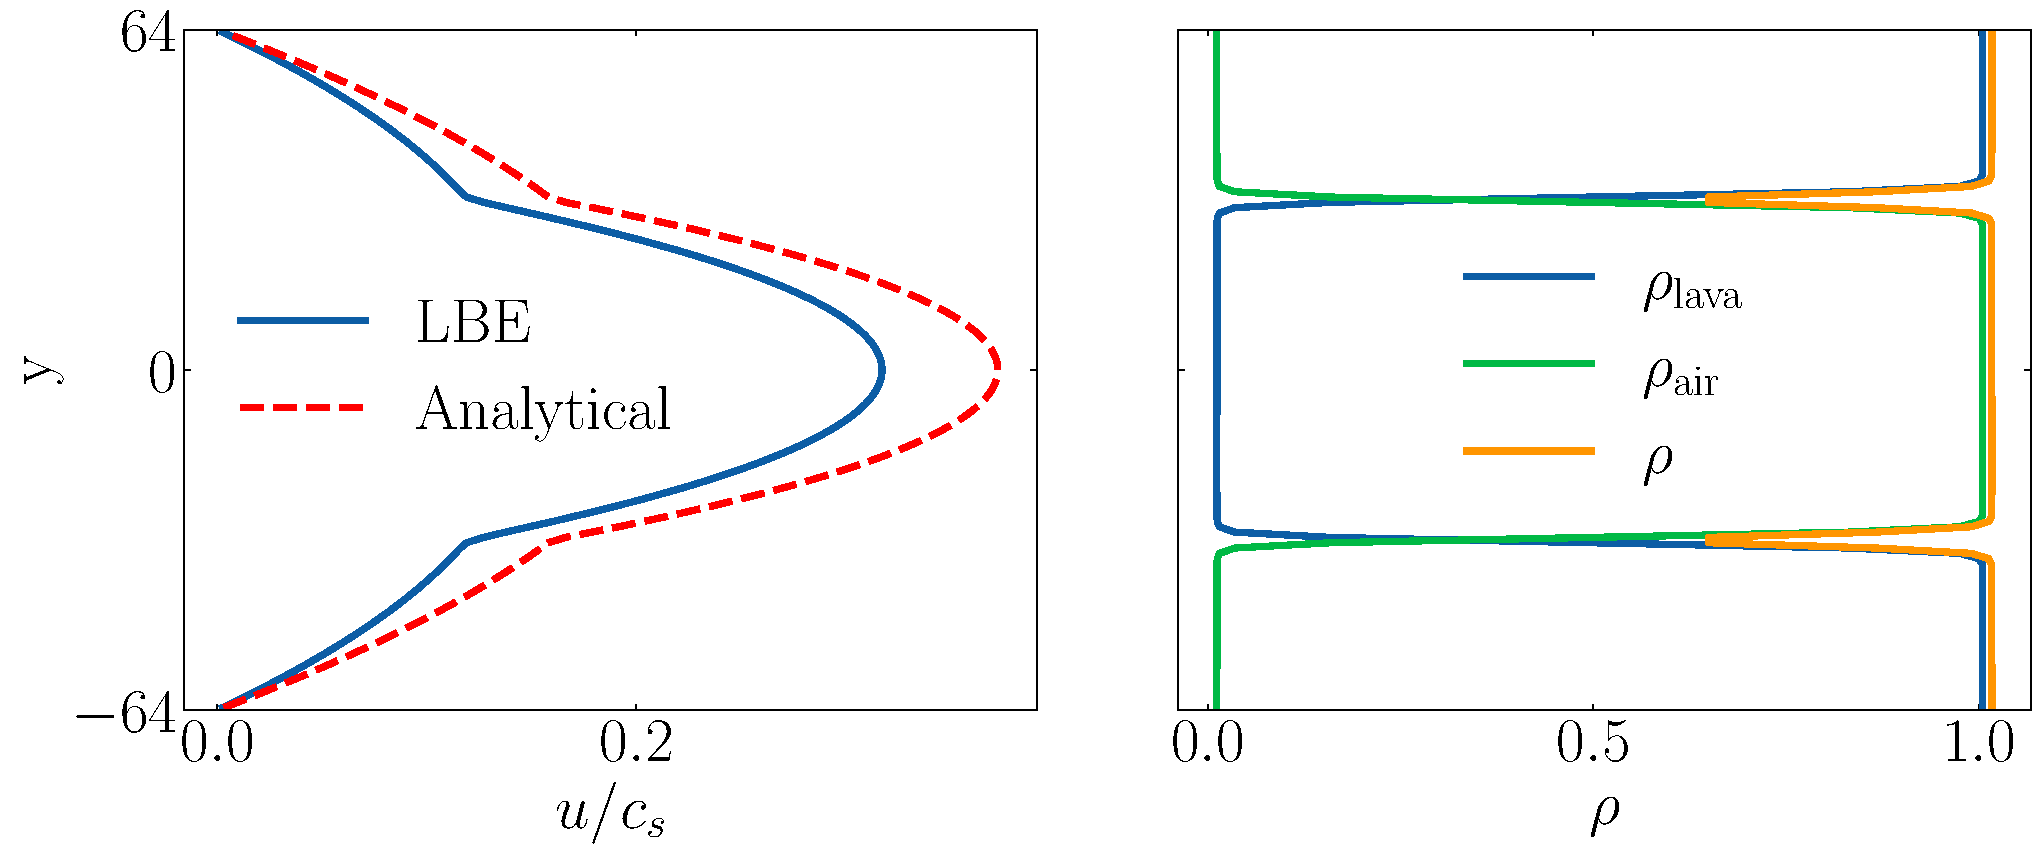
\includegraphics[width=0.9\textwidth]{figures/poiseuille_mc.pdf}
    \caption{Flow profile of simulated multicomponent Poiseuille flow at $t=10^5$ compared to the analytical solution.}\label{fig:poiseuille_mc}
\end{figure}

\subsection{Temperature}
The advection-diffusion equation for the temperature field is solved by introducing another distribution function $\bm{g}$, which gives the temperature as:

\begin{equation}
    T = \sum_i g_i
\end{equation}

The distribution function $g$ evolves according to:

\begin{equation}\label{eq:Lattice boltzmann equation temperature}
    g_i(\bm{x} + \bm{c}_i, t+1) = g_i(\bm{x}, t) - \frac{1}{\tau_g}\Bigl(g_i(\bm{x}, t) - g_i^{\text{eq}}(\bm{x}, t)\Bigr)
\end{equation}

Where the relaxation time is computed as:

\begin{equation}\label{eq:relaxation time }
    \tau_g = \frac{1}{\rho}\sum_\sigma \rho^\sigma \tau^\sigma_g
\end{equation}

Which gives the thermal diffusivity at a specific position in space as:

\begin{equation}
    \kappa = c_s^2 \left(\tau_g - \frac{1}{2}\right)
\end{equation}

And the equilibrium distribution $\bm{g}^{\text{eq}}$ is given by:

\begin{equation}
    g^{\text{eq}}_i = w_i T \left(1 + \frac{\bm{u} \cdot \bm{c}_i}{c_s^2} + \frac{{\left(\bm{u} \cdot \bm{c}_i\right)}^2}{2c_s^4} - \frac{|\bm{u}|^2}{2c_s^2}\right)
\end{equation}

The effect of the temperature field on the velocity populations comes from the buoyancy force:

\begin{equation}\label{eq:Buoyancy force}
    \bm{F}_b = -\alpha \rho_0 \left(T - T_0\right)\bm{g}
\end{equation}

Where $\alpha$ is the thermal expansion coefficient, $T_0$ is the reference temperature and $\rho_0$ is the density where the temperature is given by $T_0$. Note that the thermal expansion coefficient $\alpha$ can itself by heavily dependent on the temperature $T$. Lastly, we need to discuss the boundary conditions for the thermal populations $g$. The periodic boundary conditions are implemented in the same way as described in equation~\ref{eq:Periodic streaming step}. For the no-slip boundaries, we make use of the anti-bounce-back scheme:

\begin{equation}\label{eq:Streaming anti-bounce-back}
    g_i(\bm{x}, t+1) = -g^\ast_q(\bm{x}, t) + 2 w_q T_{\text{wall}}
\end{equation}

Where the relation between the indices $i$ and $q$ is again given by equation~\ref{eq:Bounce-back velocity component}. 

\subsection{Algorithm thermal Lattice Boltzmann}
The algorithm for a thermal fluid is given by:

\begin{itemize}\label{it:Algorithm thermal Lattice Boltzmann}
    \item[(i)] Choose $\rho(t=0)$, $\bm{u}_0$ and $T(t=0)$.
    \item[(ii)] Determine $\bm{F}_b(t=0)$.
    \item[(iii)] Compute $\bm{u}$. 
    \item[(iv)] Initialize the populations as $\bm{f}(t=0) = \bm{f}^{\text{eq}}(\rho, \bm{u})$. 
    \item[(v)] Initialize the thermal populations as $\bm{g}(t=0) = \bm{g}^{\text{eq}}(T, \bm{u})$. 
    \item[1] Calculate $\bm{g}^{\text{eq}}(T, \bm{u})$.
    \item[2] Collide the thermal populations $\rightarrow$ $\bm{g}^{\ast}$.
    \item[3] Stream the thermal populations $\rightarrow$ $\bm{g}(t + 1)$.
    \item[4] Calculate $T(t+1)$.
    \item[5] Determine $\bm{F}_b(t+1)$.
    \item[6] Calculate $\bm{f}^{\text{eq}}(\rho, \bm{u})$.
    \item[7] Calculate source $S_i$.
    \item[8] Collide the populations $\rightarrow$ $\bm{f}^{\ast}$.
    \item[9] Stream the populations $\rightarrow$ $\bm{f}(t + 1)$.
    \item[10] Calculate $\rho(t + 1)$.
    \item[11] Calculate $\bm{u}(t + 1)$.
    \item[12] $t = t + 1$ and return to step 1 while $t < t_{\text{final}}$.
\end{itemize}

\subsection{Rayleigh-Bénard convection}
We want to simulate a test case of Rayleigh-Bénard convection in a periodic channel~\cite{Rayleigh}. For this test case, we will go more deeply into the specifics of the unit conversion between real and lattice units. The chosen real length scale will be given by the height of the channel, $\widetilde{L} = \widetilde{L}_y = 1~\text{m}$. We use the buoyant velocity as the velocity scale, given by $\widetilde{U} = \sqrt{\widetilde{\alpha}\Delta\widetilde{T}\, \widetilde{g}\widetilde{L}}$. Notice that $\widetilde{\alpha}\Delta\widetilde{T}$ is a nondimensional quantitiy already. For the expansion coefficient, we arbitrarily choose $\widetilde{\alpha} = 2.07 \cdot 10^{-4}~\text{m}^2/\text{s}$. We set the bottom of the channel to $\widetilde{T}_{\text{bottom}} = 294~\text{K}$ and the top to $\widetilde{T}_{\text{top}} = 293~\text{K}$. The units of the temperature in the real case and in the lattice will be the same. The velocity scale is computed to be $\widetilde{U} \approx 4.5 \cdot 10^{-2}~\text{m}/\text{s}$. We will also choose the following dimensionless quantities:

\begin{equation}
    \textit{Ra} = \frac{\widetilde{U}^2 \widetilde{L}^2}{\nu \kappa},\quad \textit{Pr} = \frac{\nu}{\kappa}
\end{equation}

We will choose $\textit{Pr} = 0.71$, and we will vary the Rayleigh number. We will now need the relaxation times and gravitational acceleration in lattice units. To find those, we compute the conversion factors. The spatial conversion factor is computed as $C_l = \Delta \widetilde{x} / \Delta x = \Delta \widetilde{x}$ and the velocity conversion factor is given by $C_u = \widetilde{U} / U$, where we chose the velocity scale in lattice units as $U = 0.01$, such that it is much smaller than the speed of sound $c_s = \sqrt{1/3}$. The conversion factor for the diffusivities is then given by $C_\nu = C_l C_u$, and the conversion factor for acceleration is given by $C_a = C_u^2 / C_l$. 

For the grid, we choose $N_x = 100$ and $N_y = 50$, which gives $g \approx 9.7 \cdot 10^{-3}$. We do simulations for $\textit{Ra} = 5000$, $\textit{Ra} = 50000$ and $\textit{Ra} = 10^6$, where the resulting streamlines of the velocity field and contours for the temperature fields are shown in figure~\ref{fig:Rayleigh-Benard}. 

\begin{figure}[htp]

\centering

\begin{subfigure}{.8\textwidth}
    \centering
    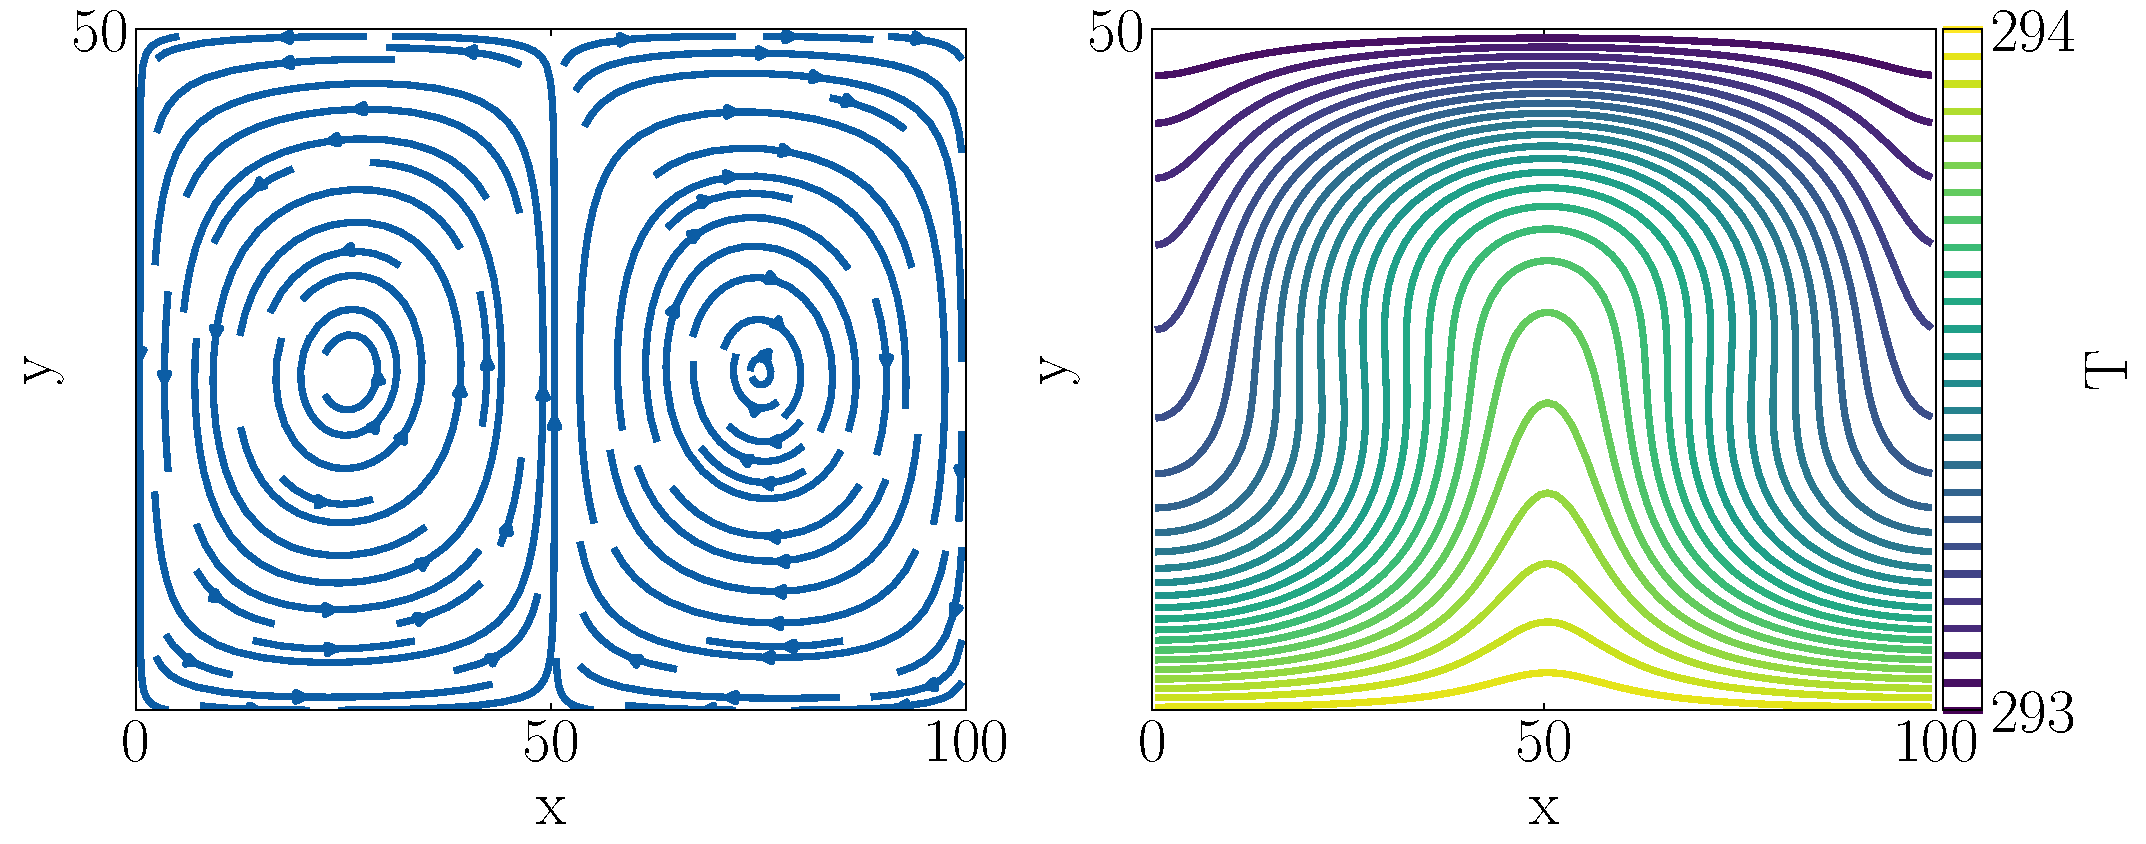
\includegraphics[width=.95\textwidth]{figures/Ra5000.pdf}
    \caption{$\textit{Ra} = 5000$}\label{fig:Ra5000}
\end{subfigure}


\bigskip

\begin{subfigure}{.8\textwidth}
    \centering
    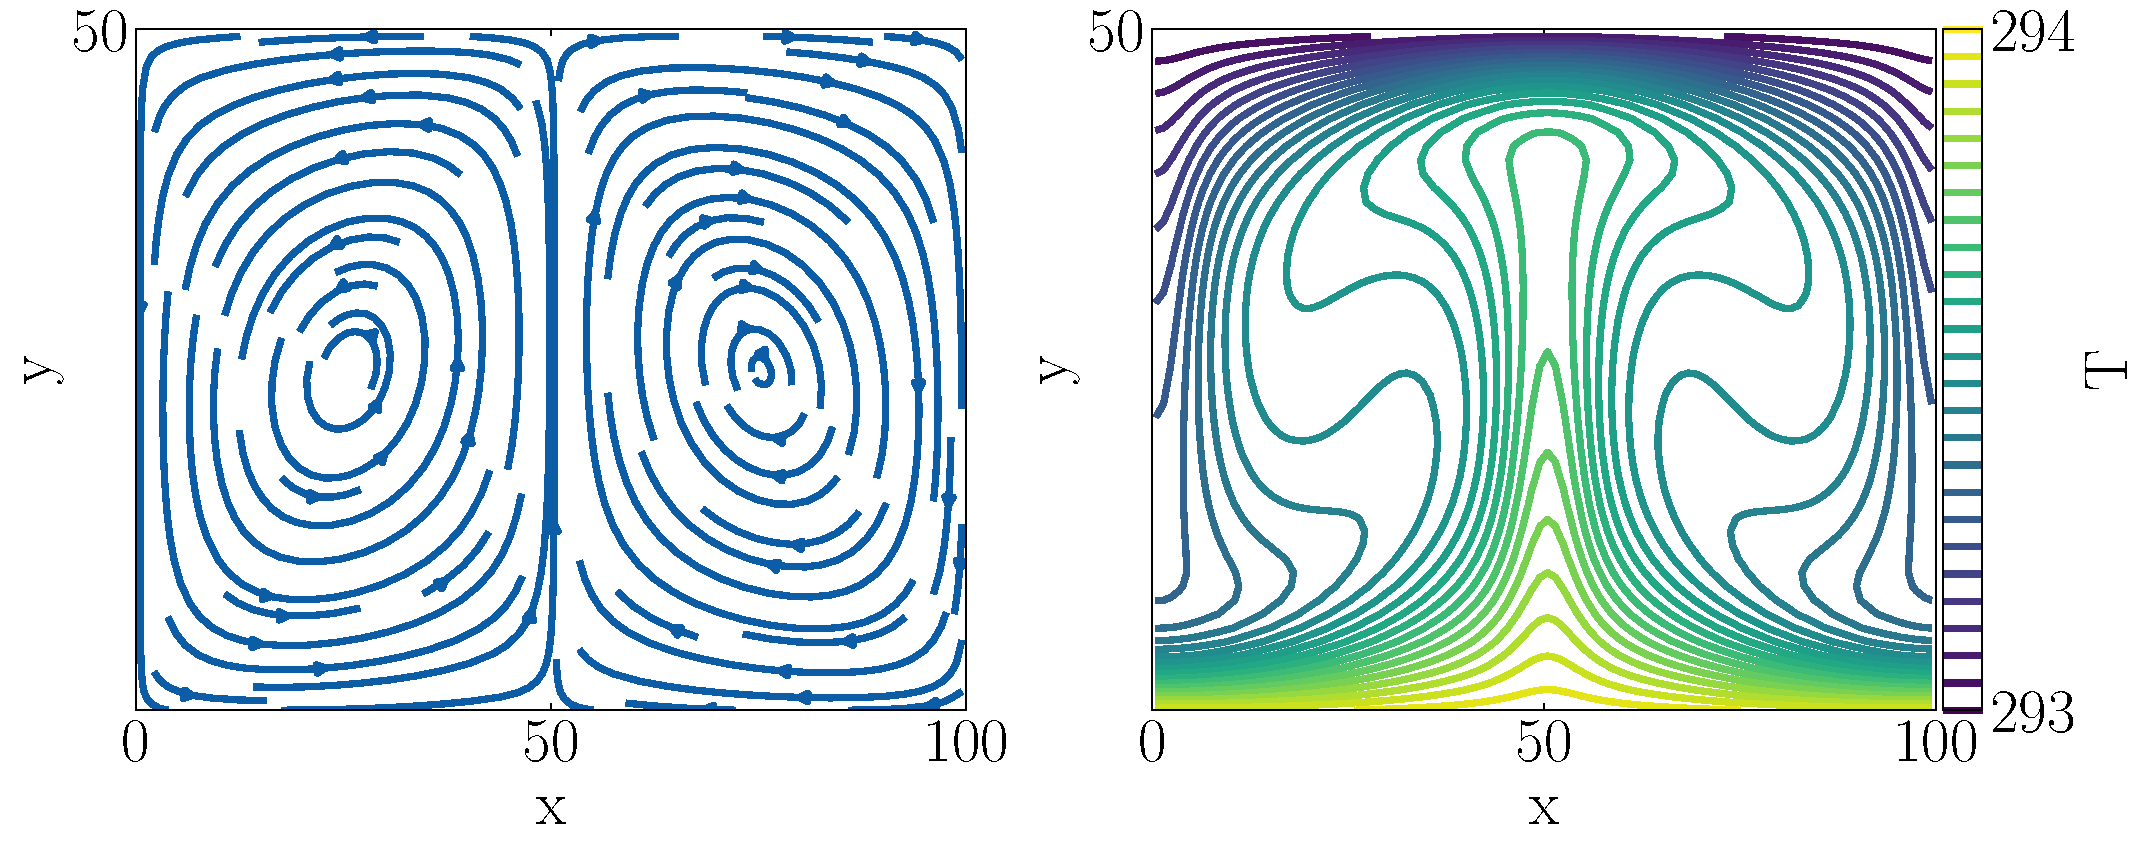
\includegraphics[width=.95\textwidth]{figures/Ra50000.pdf}
    \caption{$\textit{Ra} = 50000$}\label{fig:Ra50000}
\end{subfigure}

\bigskip

\begin{subfigure}{.8\textwidth}
    \centering
    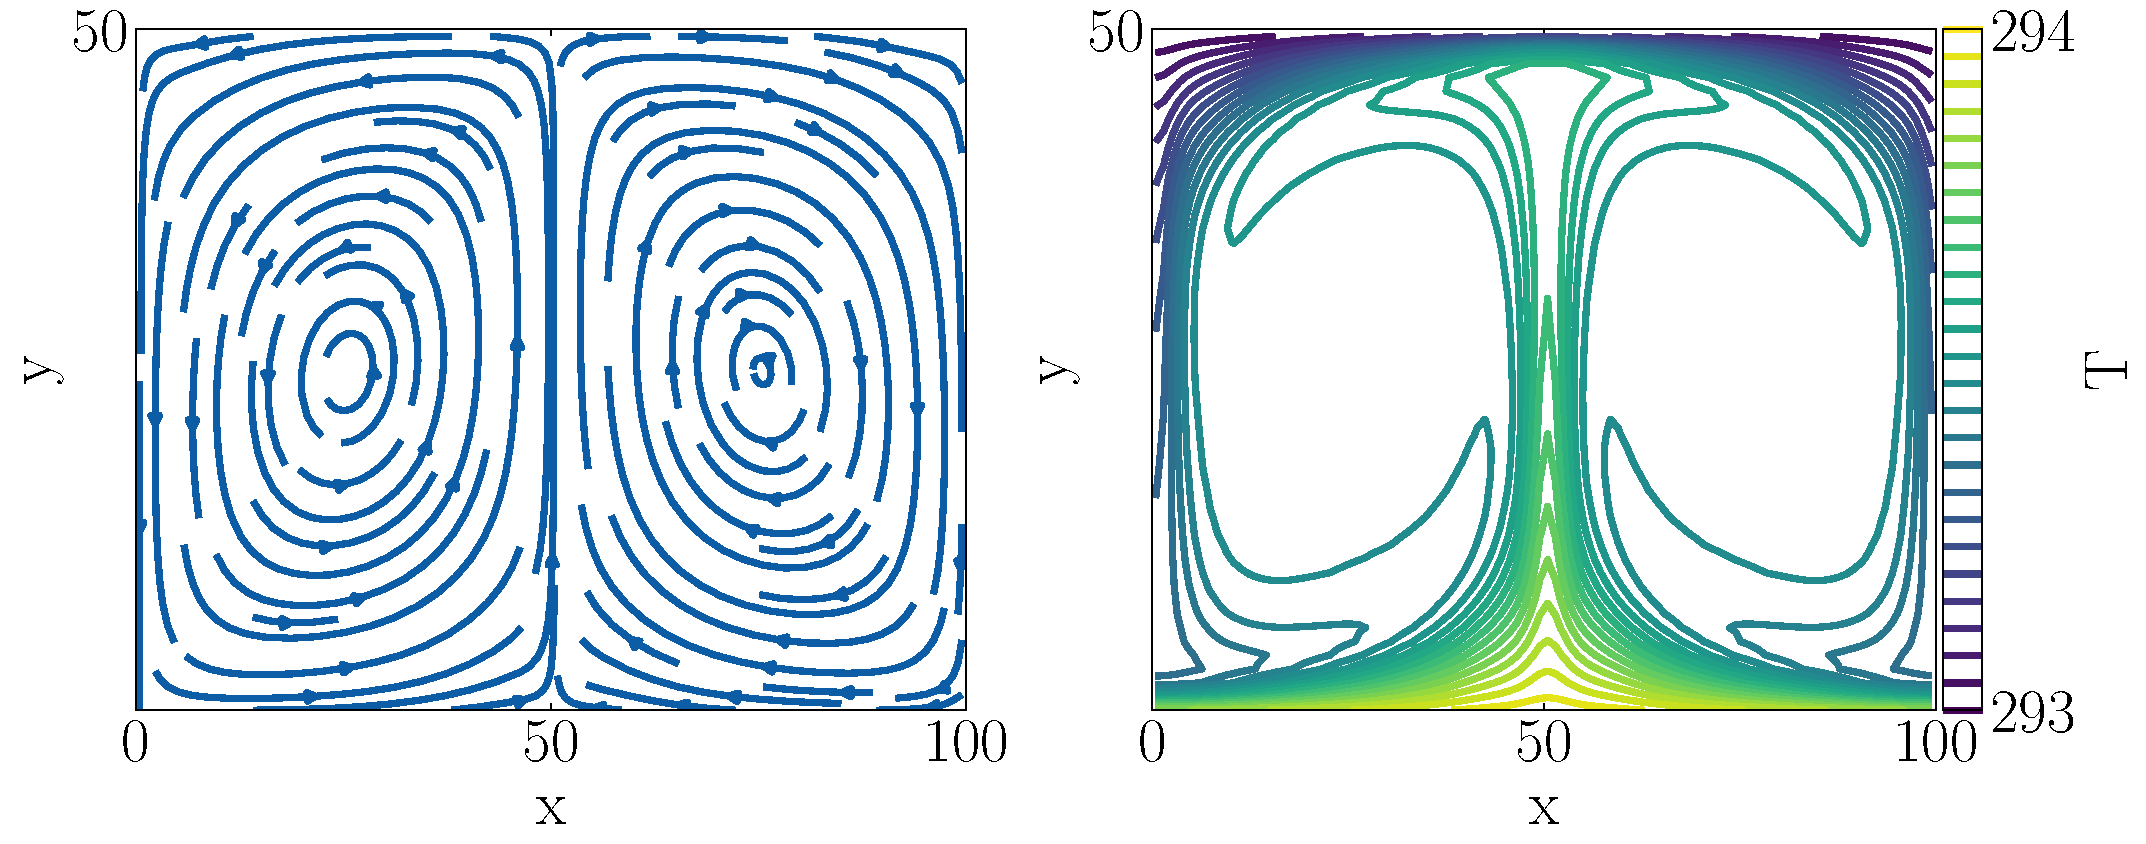
\includegraphics[width=.95\textwidth]{figures/Ra1000000.pdf}
    \caption{$\textit{Ra} = 10^6$}\label{fig:Ra1000000}
\end{subfigure}

\caption{}\label{fig:Rayleigh-Benard}
\end{figure}

\subsection{Phase change}
We want to be able to have a change of phase between liquid and solid. This is done by making use of the Enthalpy:

\begin{equation}\label{eq:Enthalpy}
    H(t) = c T(t) + L_f \phi_l(t-1)
\end{equation}

Where $H$ is the enthalpy, $c$ is the heat capacity, $L_f$ is the latent heat and $\phi_l$ is the fraction of liquid on a grid point. The heat capacity of the solid and liquid phase differs, so the term $c T(t)$ can be changed to:

\begin{equation}
    c T(t) = \left(1 - \phi_l(t-1)\right)c_{\text{solid}} T + \phi_l(t-1) \Bigl(c_{\text{liquid}} \left(T - T_m\right) + c_{\text{solid}}T_m\Bigr)
\end{equation}

The liquid fraction at time $t$ can now be computed as:

\begin{equation}
    \phi_l(t) = 
    \begin{cases}
        0, & \text{for } H(t) < H_s = c_{\text{solid}} T_m\\
        \frac{H(t)-H_s}{L_f}, & \text{for } H_s \leq H(t) \leq H_s + L_f\\
        1, & \text{for } H(t) > H_s + L_f
    \end{cases}
\end{equation}

Where $T_m$ is the melting temperature. The thermal populations at time $t+1$ can then be computed by using equation~\ref{eq:Lattice boltzmann equation temperature} with an added source:

\begin{equation}\label{eq:Lattice boltzmann equation temperature with phase change}
    g_i(\bm{x} + \bm{c}_i, t+1) = g_i(\bm{x}, t) - \frac{1}{\tau_g}\Bigl(g_i(\bm{x}, t) - g_i^{\text{eq}}(\bm{x}, t)\Bigr) - w_i \frac{L_f}{c_{\text{solid}}} \Bigl(\phi_l(\bm{x}, t)-\phi_l(\bm{x}, t-1)\Bigr)
\end{equation}

To make sure that the solid parts of the fluid stay stationary, we add a penalization force depending on the solid fraction:

\begin{equation}
    \bm{F}_{\text{pen}} = -\left(1 - \phi_l^2\right)\rho\bm{u}
\end{equation}

For the initialization fo the liquid fraction, we choose $\phi_l(t=0)$ and set $\phi_l(t=-1) = \phi_l(t=0)$. Finally, we have different thermal diffusivities for the solid and liquid phase:

\begin{equation}
    \tau_g = \phi_l \tau_g^{\text{liquid}} + \left(1 - \phi_l\right)\tau_g^{\text{solid}}
\end{equation}

\subsection{Algorithm phase change}
The algorithm for a fluid with phase change is given by:

\begin{itemize}\label{it:Algorithm phase change}
    \item[(i)] Choose $\rho(t=0)$, $\bm{u}_0$, $T(t=0)$ and $\phi_l(t=0)$.
    \item[(ii)] Set $\phi_l(t=-1) = \phi_l(t=0)$. 
    \item[(iii)] Determine $\bm{F}_b(t=0)$ and $\bm{F}_{\text{pen}}(t=0)$.
    \item[(iv)] Compute $\bm{u}$. 
    \item[(v)] Initialize the populations as $\bm{f}(t=0) = \bm{f}^{\text{eq}}(\rho, \bm{u})$. 
    \item[(vi)] Initialize the thermal populations as $\bm{g}(t=0) = \bm{g}^{\text{eq}}(T, \bm{u})$. 
    \item[1] Calculate $\bm{g}^{\text{eq}}(T, \bm{u})$. 
    \item[2] Collide the thermal populations $\rightarrow$ $\bm{g}^{\ast}$.
    \item[3] Stream the thermal populations $\rightarrow$ $\bm{g}(t + 1)$.
    \item[4] Calculate $T(t+1)$.
    \item[5] Determine $\bm{F}_b(t+1)$ and $\bm{F}_{\text{pen}}(t+1)$. 
    \item[6] Calculate $\bm{f}^{\text{eq}}(\rho, \bm{u})$.
    \item[7] Calculate source $S_i$.
    \item[8] Collide the populations $\rightarrow$ $\bm{f}^{\ast}$.
    \item[9] Stream the populations $\rightarrow$ $\bm{f}(t + 1)$.
    \item[10] Calculate $\rho(t + 1)$.
    \item[11] Calculate $\bm{u}(t + 1)$.
    \item[12] Compute $H(t+1)$ and $\phi_l(t+1)$. 
    \item[13] $t = t + 1$ and return to step 1 while $t < t_{\text{final}}$.
\end{itemize}

\subsection{Stefan problem}
To test the solidification, we apply the algorithm in~\ref{it:Algorithm phase change} to a stationary flow where we have a cold plate on the bottom below the melting temperature. This means that the interface of solidified fluid grows upwards. We define the Stefan number as:

\begin{equation}
    \textit{St} = \frac{c \Delta T}{L_f}
\end{equation}

The position of the interface over time is given by:

\begin{equation}
    y_i(t) = 2 \lambda \sqrt{\kappa t}
\end{equation}

Where the constant $\lambda$ depends on the Stefan number as:

\begin{equation}\label{eq:lambda equation}
    \lambda e^{\lambda^2} \text{erf}(\lambda) = \frac{\textit{St}}{\sqrt{\pi}}
\end{equation}

We choose $c_p^{\text{liquid}} = c_p^{\text{solid}} = 0.95$, $L_f = 1$, $\textit{St} = 1$, $T_m = 0$, $T_{\text{bottom}} = -\textit{St}/c_p^{\text{solid}}$, $T_{\text{top}} = T_m$ and $\kappa^{\text{liquid}} = \kappa^{\text{solid}} = 0.00166$. We solve equation~\ref{eq:lambda equation} by using a rootfinding algorithm. The result is given in figure~\ref{fig:stefan}.

\begin{figure}[htp]
    \centering
    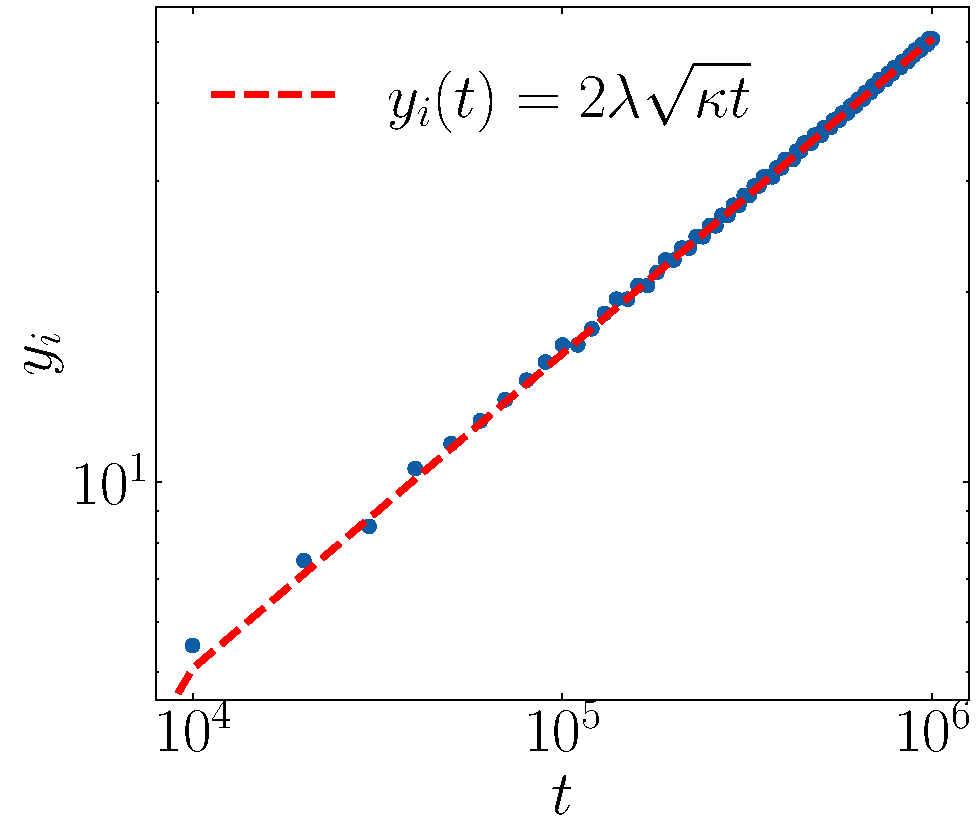
\includegraphics[width=0.5\textwidth]{figures/stefan.pdf}
    \caption{Position of interface over time, compared to the analytical solution.}\label{fig:stefan}
\end{figure}

\subsection{Phase change in multicomponent fluid}
